\documentclass{article}

%% Denote paragraphs with vertical space rather than indenting (not critical)
\usepackage{parskip}

%% Support for URL in introductory text (not needed for main example)
\usepackage{url}

%% *** Enable TikZ ***
\usepackage{tikz}

%% *** LaTeX package ***
\usepackage{braket} % LaTeX library that provides \ket

%% *** TikZ library ***
\usetikzlibrary{calc}

\begin{document}

%% Introductory Text
Example 4.7 from the book\\
\emph{Unlocking LaTeX Graphics: A Concise Guide to Ti$k$Z/PGF and PGFPLOTS}.\\
For more information, visit \url{https://latex-graphics.com}.
\par\bigskip

%% *** START OF EXAMPLE CODE ***
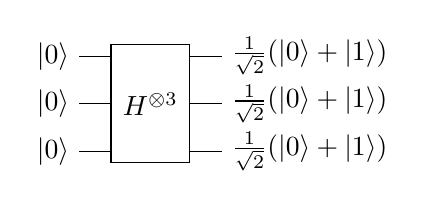
\begin{tikzpicture}
  \node[minimum height=1.5cm,minimum width=1cm,draw] (H) {$H^{\otimes 3}$};
  \foreach \val in {0.1,0.5,0.9} {
    \draw ($(H.north west)!\val!(H.south west)$) --
      ++(-0.4,0) node[left] {$\ket{0}$};
    \draw ($(H.north east)!\val!(H.south east)$) --
      ++(0.4,0) node[right] {$\frac{1}{\sqrt{2}} (\ket{0} + \ket {1})$}; }
\end{tikzpicture}
%% *** END OF EXAMPLE CODE ***

\end{document}
